\documentclass{article}
\pdfpagewidth=8.5in
\pdfpageheight=11in
\usepackage{ijcai22}

\usepackage{times}
\renewcommand*\ttdefault{txtt}
\usepackage{soul}
\usepackage{url}
\usepackage[hidelinks]{hyperref}
\usepackage[utf8]{inputenc}
\usepackage[small]{caption}
\usepackage{graphicx}
\usepackage{amsmath}
\usepackage{booktabs}
 \usepackage{hyperref}
\usepackage[
backend=biber,
style=alphabetic,
]{biblatex}
\urlstyle{same}


\title{PoseGTAC: Graph Transformer Encoder-Decoder with Atrous Convolution for 3D Human Pose Estimation}

\author{
Yiran Zhu\and
Xing Xu\footnote{Corresponding author}\and
Fumin Shen\and
Yanli Ji\and
Lianli Gao\And
Heng Tao Shen\\
\affiliations
Center for Future Media & School of Computer Science and Engineering\\
University of Electronic Science and Technology of China, China\\
\emails
\{yiranupup, fumin.shen\}@gmail.com,
\{xing.xu, yanliji, lianli.gao\}@uestc.edu.cn, shenhengtao@hotmail.com
}

\addbibresource{ref.bib}

\begin{document}

\maketitle
\begin{abstract}
Graph neural networks (GNNs) have been widely used in the 3D human pose estimation task, since the pose representation of a human body can be naturally modeled by the graph structure. Generally, most of the existing GNN-based models utilize the restricted receptive fields of filters and single-scale information, while neglecting the valuable multiscale contextual information. To tackle this issue, we propose a novel model named \textit{Graph Transformer Encoder-Decoder with Atrous Convolution} (PoseGTAC), to effectively extract multi-scale context and long-range information. Specifically, our PoseGTAC model has two key components: Graph Atrous Convolution (GAC) and Graph Transformer Layer (GTL), which are respectively for the extraction of local multi-scale and global long-range information. They are combined and stacked in an encoder-decoder structure, where graph pooling and unpooling are adopted for the interaction of multi-scale information from local to global aspect (\textit{e.g.}, part-scale and body-scale). Extensive experiments on the Human3.6M and MPI-INF-3DHP datasets demonstrate that the proposed PoseGTAC model achieves state-of-the-art performance.
\end{abstract}

\section{Introduction}

In recent years, 3D human pose estimation is attracting intensive attention in various human-related research fields, such as action recognition \cite{Yan et al., 2018, Ji et al., 2019}, human-object interaction \cite{Li et al., 2020} and motion prediction \cite{Mao et al., 2019}. Its goal is to estimate 3D coordinates of human body joints from 2D poses or images. Compared with the methods \cite{Zhou et al., 2017, Wu and Xiao, 2020} using RGB images, the 2D-to-3D methods \cite{Zhao et al., 2019, Liu et al., 2020} using only 2D poses can avoid the influence of background noise and greatly reduce the computational complexity, thus achieving competitive performance.

\begin{figure}
    \centering
    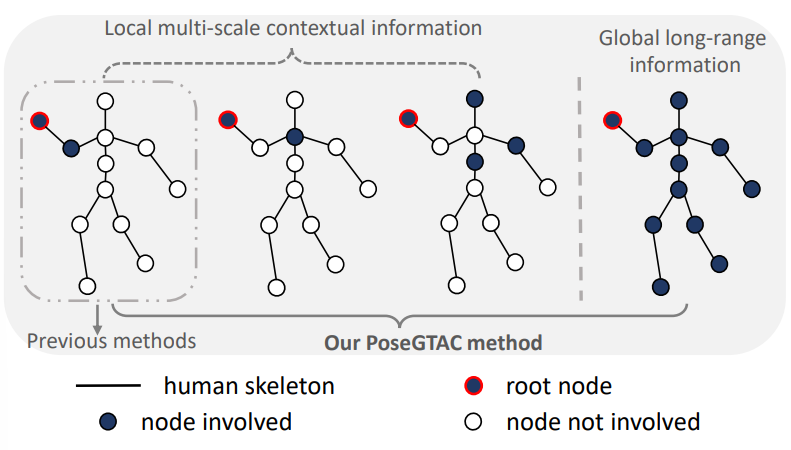
\includegraphics[width=0.45\textwidth]{figures/Fig1.png}
    \caption{Previous methods commonly adopt the restricted receptive fields of filters and ignore various multi-scale contextual information. Differently, our proposed PoseGTAC method enlarges the receptive fields of filters for capturing multi-scale context.}
\end{figure}

\begin{table}[]
\centering
\begin{tabular}{l|c}
\hline
Method & MPJPE (mm) ↓\\
\hline
SemGCN [Zhao \textit{et al.}, 2019] & 43.8\\
with GAC & 38.9\\
with GTL & 39.4\\
with GAC GTL & 38.6\\
PoseGTAC (Ours) & 38.2\\
\hline
\end{tabular}
\caption{Ablation study on the Human3.6M dataset for the MPJPE between the predicted pose and the ground-truth.}
\end{table}


\begin{equation}
\textbf{X}^{(i+1)}=\sigma(\textbf{WX}^{(i)}(\Lambda \odot \textbf{M})),
\end{equation}

\medskip

\printbibliography

\end{document}

